\section{Internal Block Diagram - BMS}
Due to the complexity of the Battery Management System its interconnectivity has been visualized on a seperate Internal Block Diagram. The result is seen below.
\fxnote{analog front end - JOnathan}
\begin{figure}[H]
	\centering
	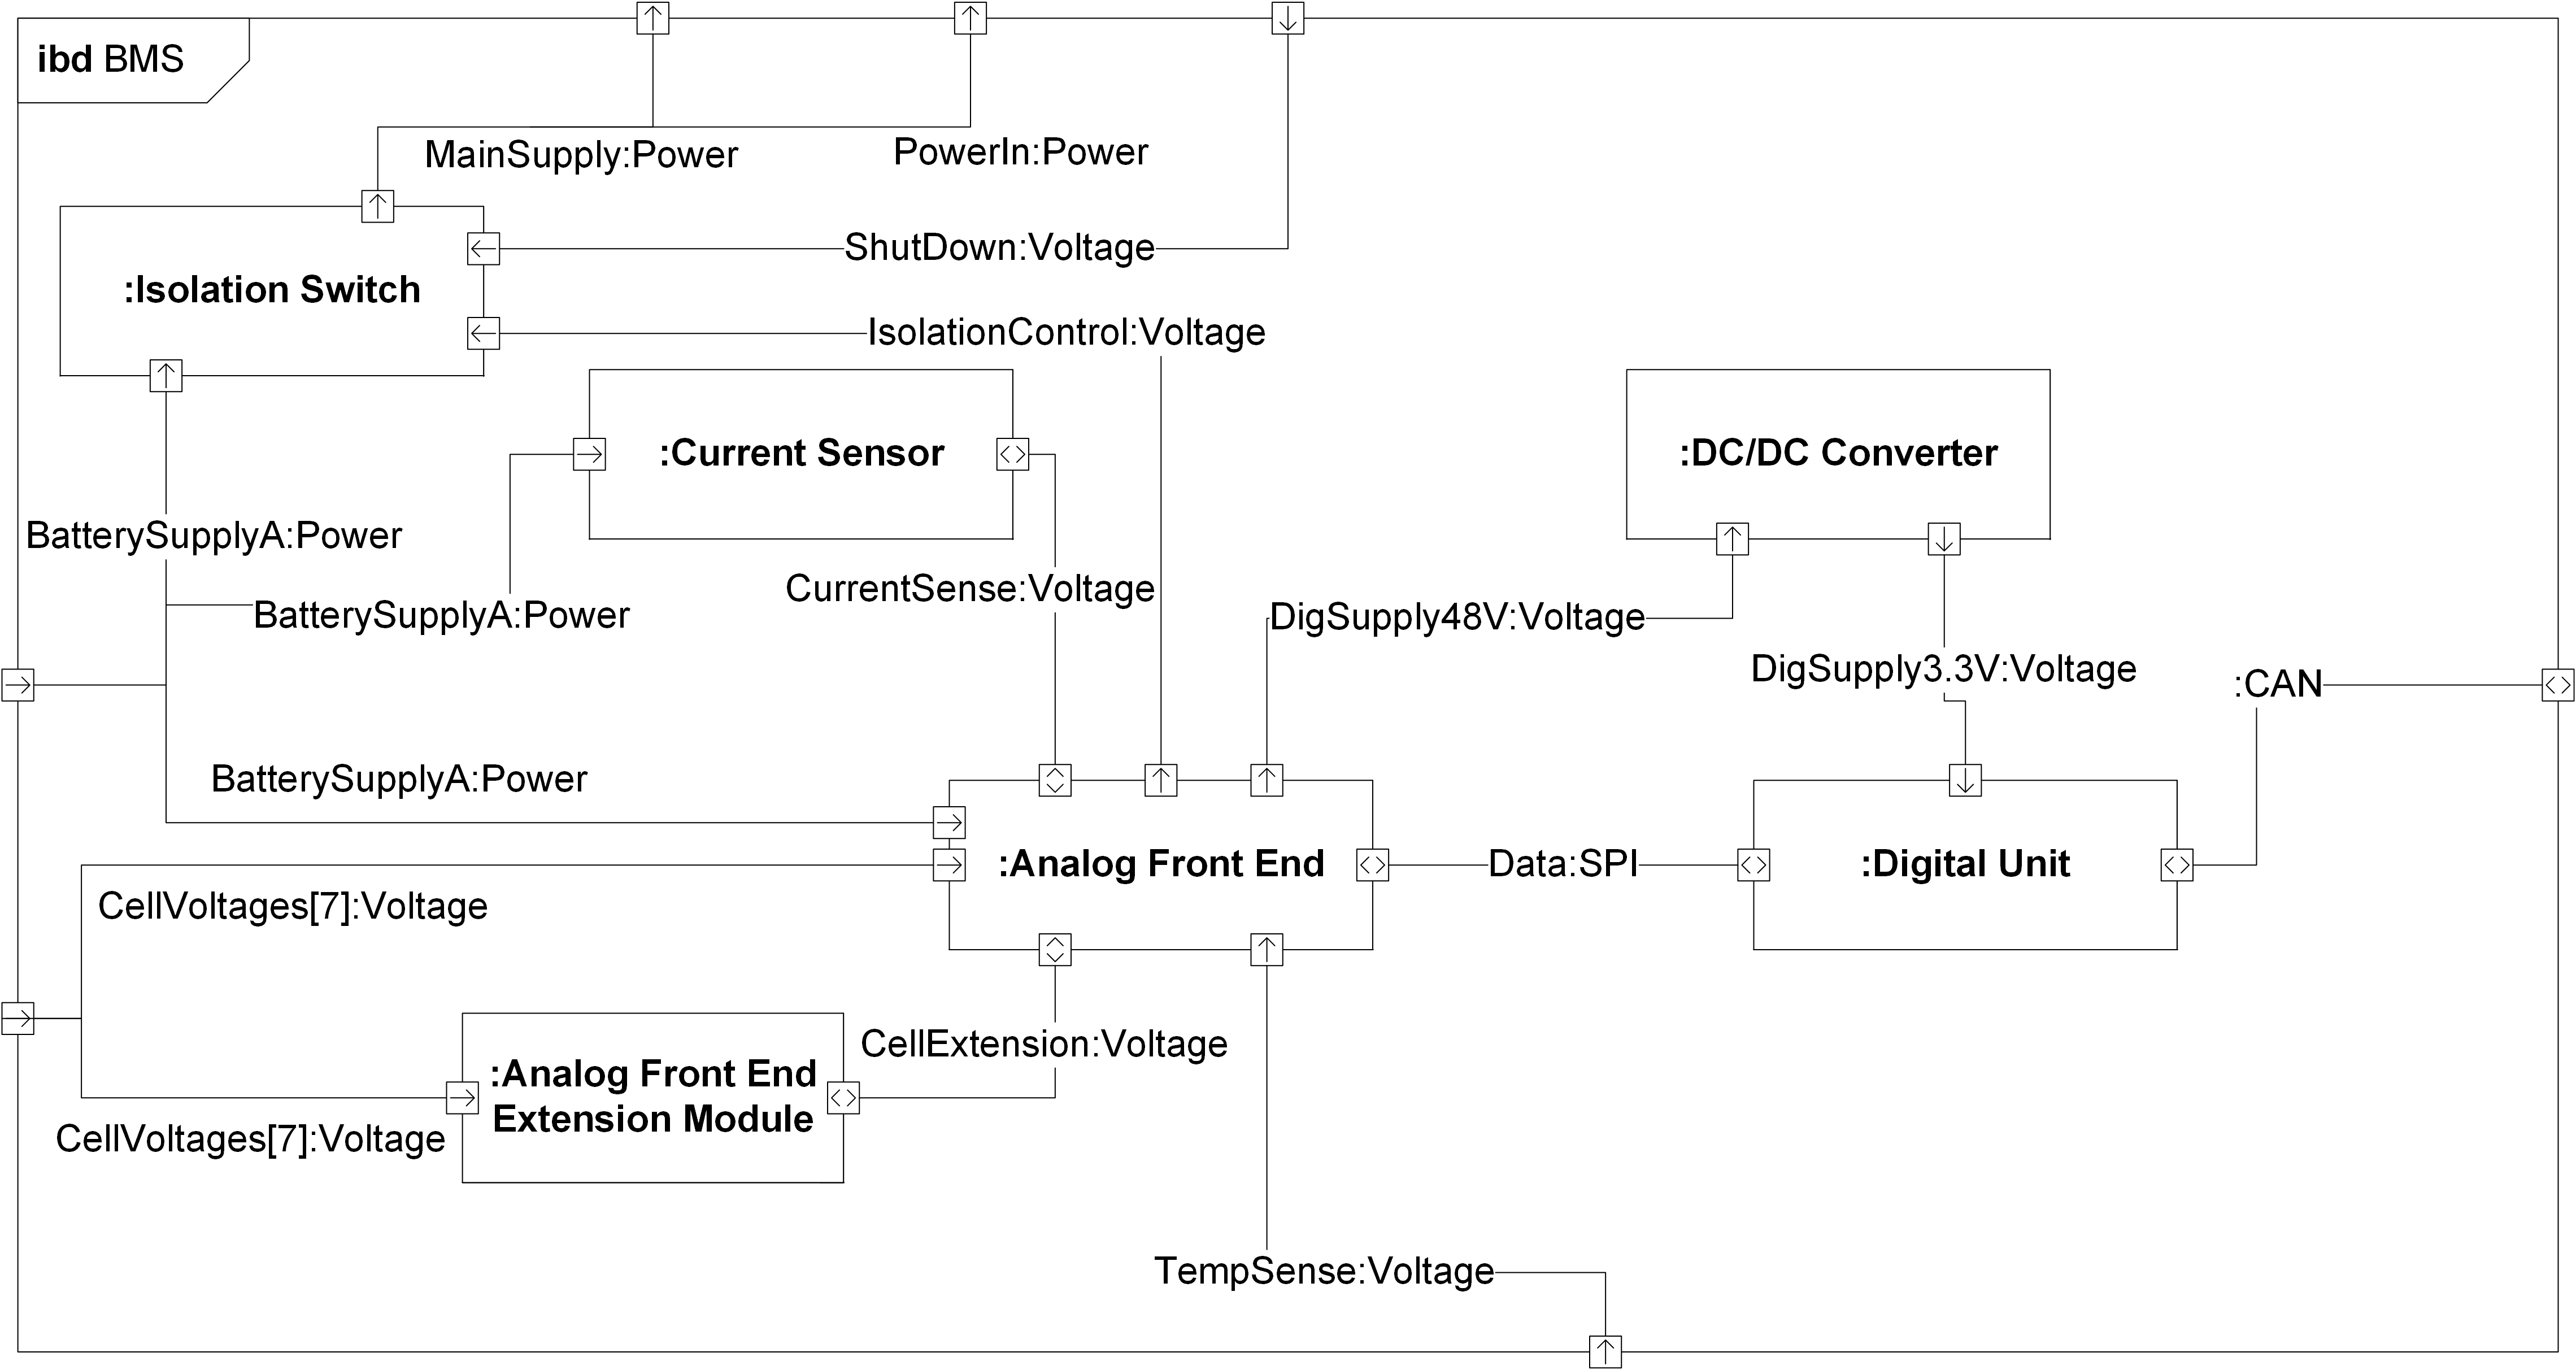
\includegraphics[width=1\linewidth]{Architecture/Diagrams/IBD_BMS}
	\caption{IBD for AU2's Battery Management System}
	\label{fig:IBD_BMS}
\end{figure}

\section{Signal description - BMS}
The signals and protocols used to communicate between the blocks in BMS are specified in this section.

\textbf{Block :BMS}\\
Block interface description:
\begin{itemize}
	\item \textbf{ShutDown:Voltage}\\
	Direction: [External] $\rightarrow$ [Analog Unit]\\
	Description: Shuts down the system if a change in the voltage-level is measured.
	\item \textbf{MainSupply:Power}\\
	Direction: [External] $\rightarrow$ [Analog Unit]\\
	Description: The power from the battery which is delivered to the remaining electrical systems in the car.
	\item \textbf{BMSC:CAN}\\
	Direction: [External] $\leftrightarrow$ [Digital Unit]\\
	Description: CAN-communication with a computer in order to gain information about various variables.
	\item \textbf{BatterySupplyA:Power}\\
	Direction: [External] $\rightarrow$ [Current Sensor]\\
	Description: Power directly from the battery before being measured by the current sensor.
	\item \textbf{AnSupply:Voltage}\\
	Direction: [External] $\rightarrow$ [Analog Unit]\\
	Description: Power supply for the analog part of the system.
	\item \textbf{TempSense:Voltage}\\
	Direction: [External] $\rightarrow$ [Analog Unit]\\
	Description: A voltage which is proportional to the battery's temperature.
\end{itemize}

\textbf{Block :Current Sensor}\\
Block interface description:
\begin{itemize}
	\item \textbf{BatterySupplyA:Power}\\
	Direction: [Battery] $\rightarrow$ [Current Sensor]\\
	Description: Power directly from the battery before being measured by the current sensor.
	\item \textbf{BatterySupplyB:Power}\\
	Direction: [Current Sensor] $\rightarrow$ [Analog Unit]\\
	Description: Power directly from the battery after being measured by the current sensor.
	\item \textbf{CurrentSense:Voltage}\\
	Direction: [Current Sensor] $\rightarrow$ [Analog Unit]\\
	Description: A voltage which is proportional to the output current from the battery.
\end{itemize}

\textbf{Block :Analog Unit}\\
Block interface description:
\begin{itemize}
	\item \textbf{AnSupply:Voltage}\\
	Direction: [Battery] $\rightarrow$ [Analog Unit]\\
	Description: Power supply for the analog part of the system.
	\item \textbf{BatterySupplyB:Power}\\
	Direction: [Current Sensor] $\rightarrow$ [Analog Unit]\\
	Description: Power directly from the battery after being measured by the current sensor.
	\item \textbf{CurrentSense:Voltage}\\
	Direction: [Current Sensor] $\rightarrow$ [Analog Unit]\\
	Description: A voltage which is proportional to the output current from the battery.
	\item \textbf{ShutDown:Voltage}\\
	Direction: [External] $\rightarrow$ [Analog Unit]\\
	Description: Shuts down the system if a change in the voltage-level is measured.
	\item \textbf{Error:SPI}\\
	Direction: [Analog Unit] $\leftrightarrow$ [Digital Unit]\\
	Description: Sends the measured analog data to the digital unit in order to be sent to a computer.
	\item \textbf{DigSupply:Voltage}\\
	Direction: [Analog Unit] $\rightarrow$ [Digital Unit]\\
	Description: Power supply for the digital part of the system.
	\item \textbf{MainSupply:Power}\\
	Direction: [External] $\rightarrow$ [Analog Unit]\\
	Description: The power from the battery which is delivered to the remaining electrical systems in the car.
	\item \textbf{TempSense:Voltage}\\
	Direction: [Battery] $\rightarrow$ [Analog Unit]\\
	Description: A voltage which is proportional to the battery's temperature.
\end{itemize}

\textbf{Block :Digital Unit}\\
Block interface description:
\begin{itemize}
	\item \textbf{Error:SPI}\\
	Direction: [Analog Unit] $\leftrightarrow$ [Digital Unit]\\
	Description: Sends the measured analog data to the digital unit in order to be sent to a computer.
	\item \textbf{BMSC:CAN}\\
	Direction: [External] $\leftrightarrow$ [Digital Unit]\\
	Description: CAN-communication with a computer in order to gain information about various variables.
	\item \textbf{DigSupply:Voltage}\\
	Direction: [Analog Unit] $\rightarrow$ [Digital Unit]\\
	Description: Power supply for the digital part of the system.
\end{itemize}

